% !TEX root       = ./type_name.tex
% !TEX program    = pdflatex
% !TEX encoding   = utf-8
% !TEX spellcheck = de_DE_frami
%=======================================================================

\chapter{Further possible extensions in OpenStack}\label{ch:futurepossibilities}
Being one of the key open source software platform for Cloud Computing in Infrastructure-as-a-Service model, it has various possible implementations and extensions.
As far as networking is concerned, there are modules in and out of OpenStack which provides the Network Functions Virtualization (NFV) for global telecom providers.

Network Functions Virtualization (NFV) allows telecom and enterprise network operators to control their networking functions: physical, virtual and functional domains—using commercial off-the-shelf hardware, and open source software as a single control pane for management and orchestration.
Here, OpenStack can provide a platform for the development and evolution of NFV components across the virtual systems. With robust system level integration and deployment a reference NFV platform can be created to accelerate the transformation of enterprise and service provider networks.

Early on, the telecommunications industries and the networking vendors have recognised the potential for OpenStack as a platform for NFV, which triggered investigations and work in development of OpenStack compatible modules to optimize for NFV.

"Network Functions Virtualization (NFV) is now synonymous with OpenStack. When people say NFV, there is an implication that they are talking about OpenStack."\cite{openstack_nfv}

Both the European Telecommunications Standards Institute and Linux Foundation collaboration project OPNFV have defined specifications and released reference platforms for NFV that select OpenStack as the Virtualization Infrastructure Manager. Additionally, OpenStack is the dominant choice for additional management and orchestration functions.\cite{nfv_technical_overview}

The interoperability between OpenStack and virtualized network functions is still an ongoing development.

So, what does Network Functions Virtualization (NFV) define?
To answer in a simple way, it is a new way to define, create, and manage networks by replacing dedicated network appliances with software and automation.
It is the idea of replacing the physical network devices which are dedicated and expensive by the virtual software devices.

\begin{figure}[H]
	\begin{center}
		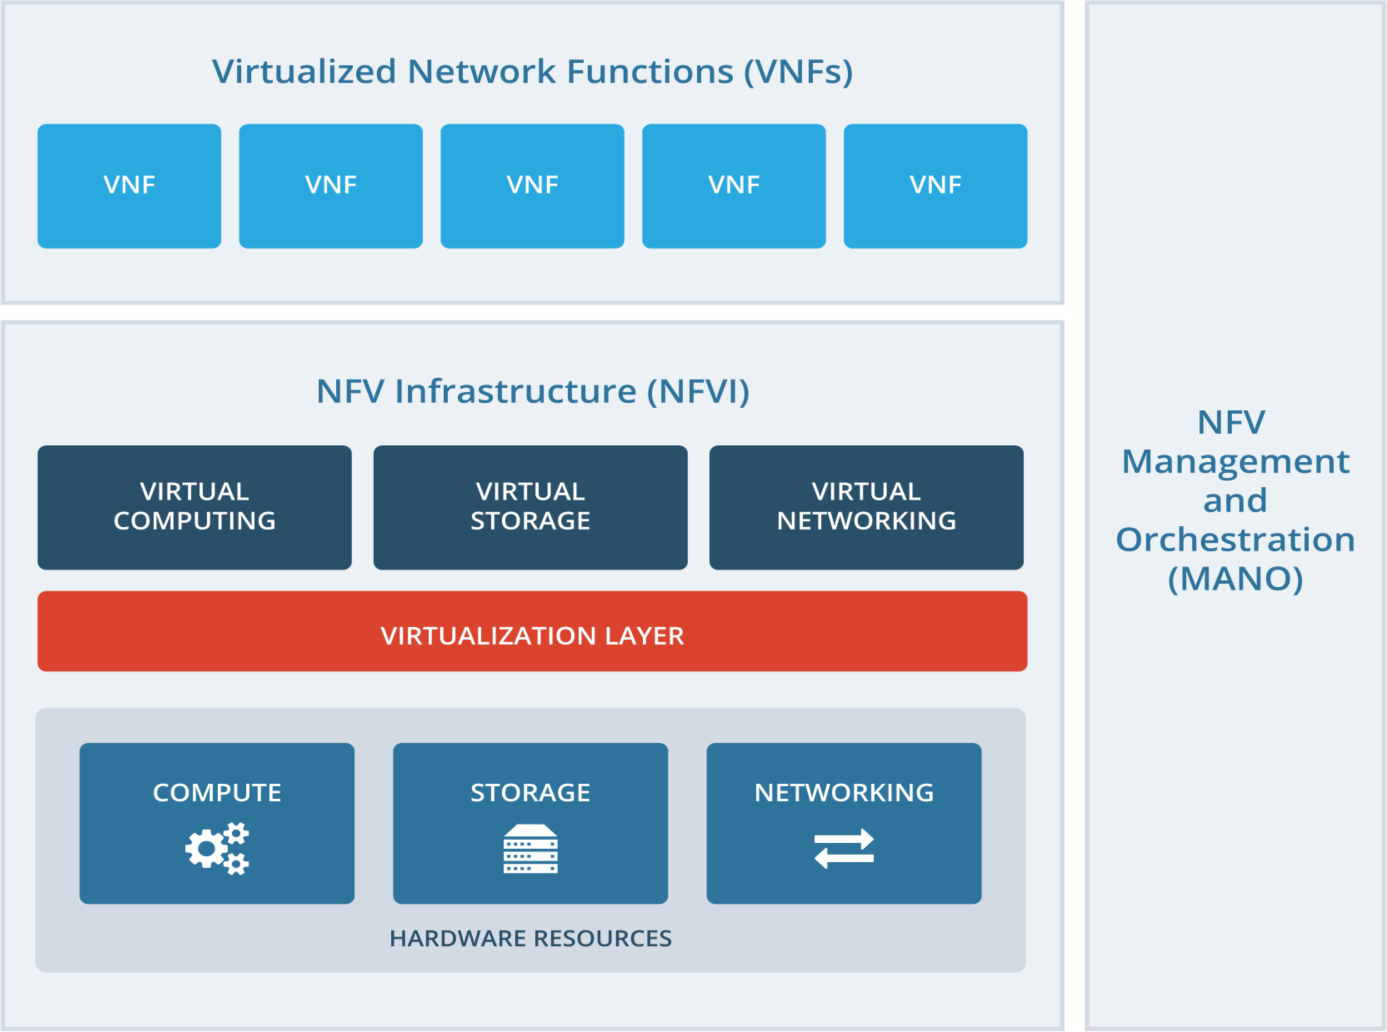
\includegraphics[width=1\linewidth]{OpenStackFoundationNFVReport}
		\caption{NFV functional overview\cite{openstack_nfv}}
		\label{fig:OpenStackFoundationNFVReport}
	\end{center}
	\vspace{-10pt}
\end{figure}

In an NFV environment, a virtual network function (VNF) takes on the responsibility of handling specific network functions that run on one or more virtual machines (VMs), on bare metal, or in containers, on top of the physical networking infrastructure.
A VNF can be an instance of any virtual hardware, for example: message router, CDN, DPI, Firewall, DNS...

The benefits of NFV stem from the fact that it runs on general purpose servers and switches in virtual machines or containers and is built with standard open APIs.

There are many ongoing NFV implementations. To keep it short, two of the NFV projects will be discussed.
\begin{itemize}
	\item Open Baton
	\item Tacker
\end{itemize}

\section{Open Baton - NFV Orchestrator}\label{sec:openbaton}
Open Baton is an European Telecommunications Standards Institute's (ETSI) NFV compliant Management and Orchestration (MANO) Framework.
It enables virtual Network Services deployments on top of the NFV infrastructure.

\begin{figure}[H]
	\begin{center}
		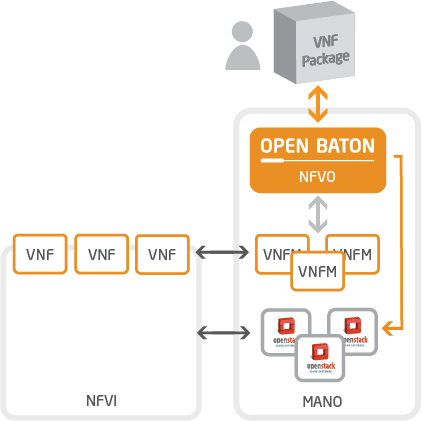
\includegraphics[width=1\linewidth]{openbaton_openstack}
		\caption{Placement of VNFM and VNF over the OpenStack Vitual Machines\cite{openBatonFeatures}}
		\label{fig:openbaton_openstack}
	\end{center}
	\vspace{-10pt}
\end{figure}

The Open Baton software is deployed over OpenStack with its own dashboard which would provide an easy to use web based VNF management console.
The VNF is configured on the virtual machine in the OpenStack IaaS.


\section{Tacker - OpenStack NFV Orchestration}\label{sec:tacker}

Tacker is an official OpenStack project building a Generic VNF Manager (VNFM) and a NFV Orchestrator (NFVO) to deploy and operate Network Services and Virtual Network Functions (VNFs) on an NFV infrastructure platform like OpenStack. It is based on ETSI MANO Architectural Framework and provides a functional stack to Orchestrate Network Services end-to-end using VNFs.

